\begin{frame}
  \frametitle{Cascaded Differential Equations}

  \begin{flushright}
    \textbf{Antti Honkela}
  \end{flushright}
  \begin{itemize}
  \item Transcription factor protein also has governing mRNA.
  \item This mRNA can be measured.
  \item In signalling systems this measurement can be misleading because it
    is activated (phosphorylated) transcription factor that counts.
  \item In development phosphorylation plays less of a role.
  \end{itemize}

\end{frame}

\begin{frame}
  \frametitle{Drosophila \emph{Mesoderm} Development}

  \textbf{Data from Furlong Lab in EMBL Heidelberg.}
  \begin{itemize}
  \item Describe mesoderm development.
  \end{itemize}

\end{frame}

\begin{frame}
  \frametitle{Cascaded Differential Equations }

  \begin{flushright}
    \textbf{Antti Honkela}
    \par\end{flushright}

  We take the production rate of active transcription factor to be given
  by \begin{align*}
    \frac{\text{d}\tfConcentration\left(t\right)}{\text{d}t} & =\sigma \tfMrnaConcentration\left(t\right)-\delta \tfConcentration\left(t\right)\\
    \frac{\text{d}\mrnaConcentration_{j}\left(t\right)}{\text{d}t} & =\basalRate_{j}+\sensitivity_{j}\tfConcentration\left(t\right)-\decayRate_{j}\mrnaConcentration_{j}\left(t\right)\end{align*}
  The solution for $\tfConcentration(t)$, setting transient terms to zero, is \[
  \tfConcentration(t)=\sigma\exp\left(-\delta t\right)\int_{0}^{t}\tfMrnaConcentration(u)\exp\left(\delta u\right)\text{d}u\ .\]



\end{frame}

\begin{frame}
  \frametitle{Covariance for Translation/Transcription Model}

  \textbf{RBF covariance function for $\tfMrnaConcentration\left(t\right)$}

  \begin{center}
    {\footnotesize \begin{eqnarray*}
        \tfConcentration\left(t\right) & = & \sigma\exp\left(-\delta t\right)\int_{0}^{t}\tfMrnaConcentration(u)\exp\left(\delta u\right)\text{d}u\\
        \mrnaConcentration_{i}\left(t\right) & = & \frac{\basalRate_{i}}{\decayRate_{i}}+\sensitivity_{i}\exp\left(-\decayRate_{i}t\right)\int_{0}^{t}\tfConcentration\left(u\right)\exp\left(\decayRate_{i}u\right)\text{d}u.\end{eqnarray*}
    }
    \par\end{center}{\footnotesize \par}

  \vspace{-2cm}

  \begin{columns}[c]


    \column{4cm}
    \begin{itemize}
    \item Joint distribution for $\mrnaConcentration_{1}\left(t\right)$, $\mrnaConcentration_{2}\left(t\right)$,
      $\tfConcentration\left(t\right)$ and $\tfMrnaConcentration\left(t\right)$.
    \item Here:\vspace{0.1cm}


      {\small }\begin{tabular}{|c|c|c|c|c|}
        \hline 
        $\delta$ & {\small $\decayRate_{1}$} & {\small $\sensitivity_{1}$} & {\small $\decayRate_{2}$} & {\small $\sensitivity_{2}$}\tabularnewline
        \hline
        \hline 
        0.1 & 5 & {\small 5} & {\small 0.5} & {\small 0.5}\tabularnewline
        \hline
      \end{tabular}{\small \par}

    \end{itemize}

    \column{6cm}

    \begin{center}
      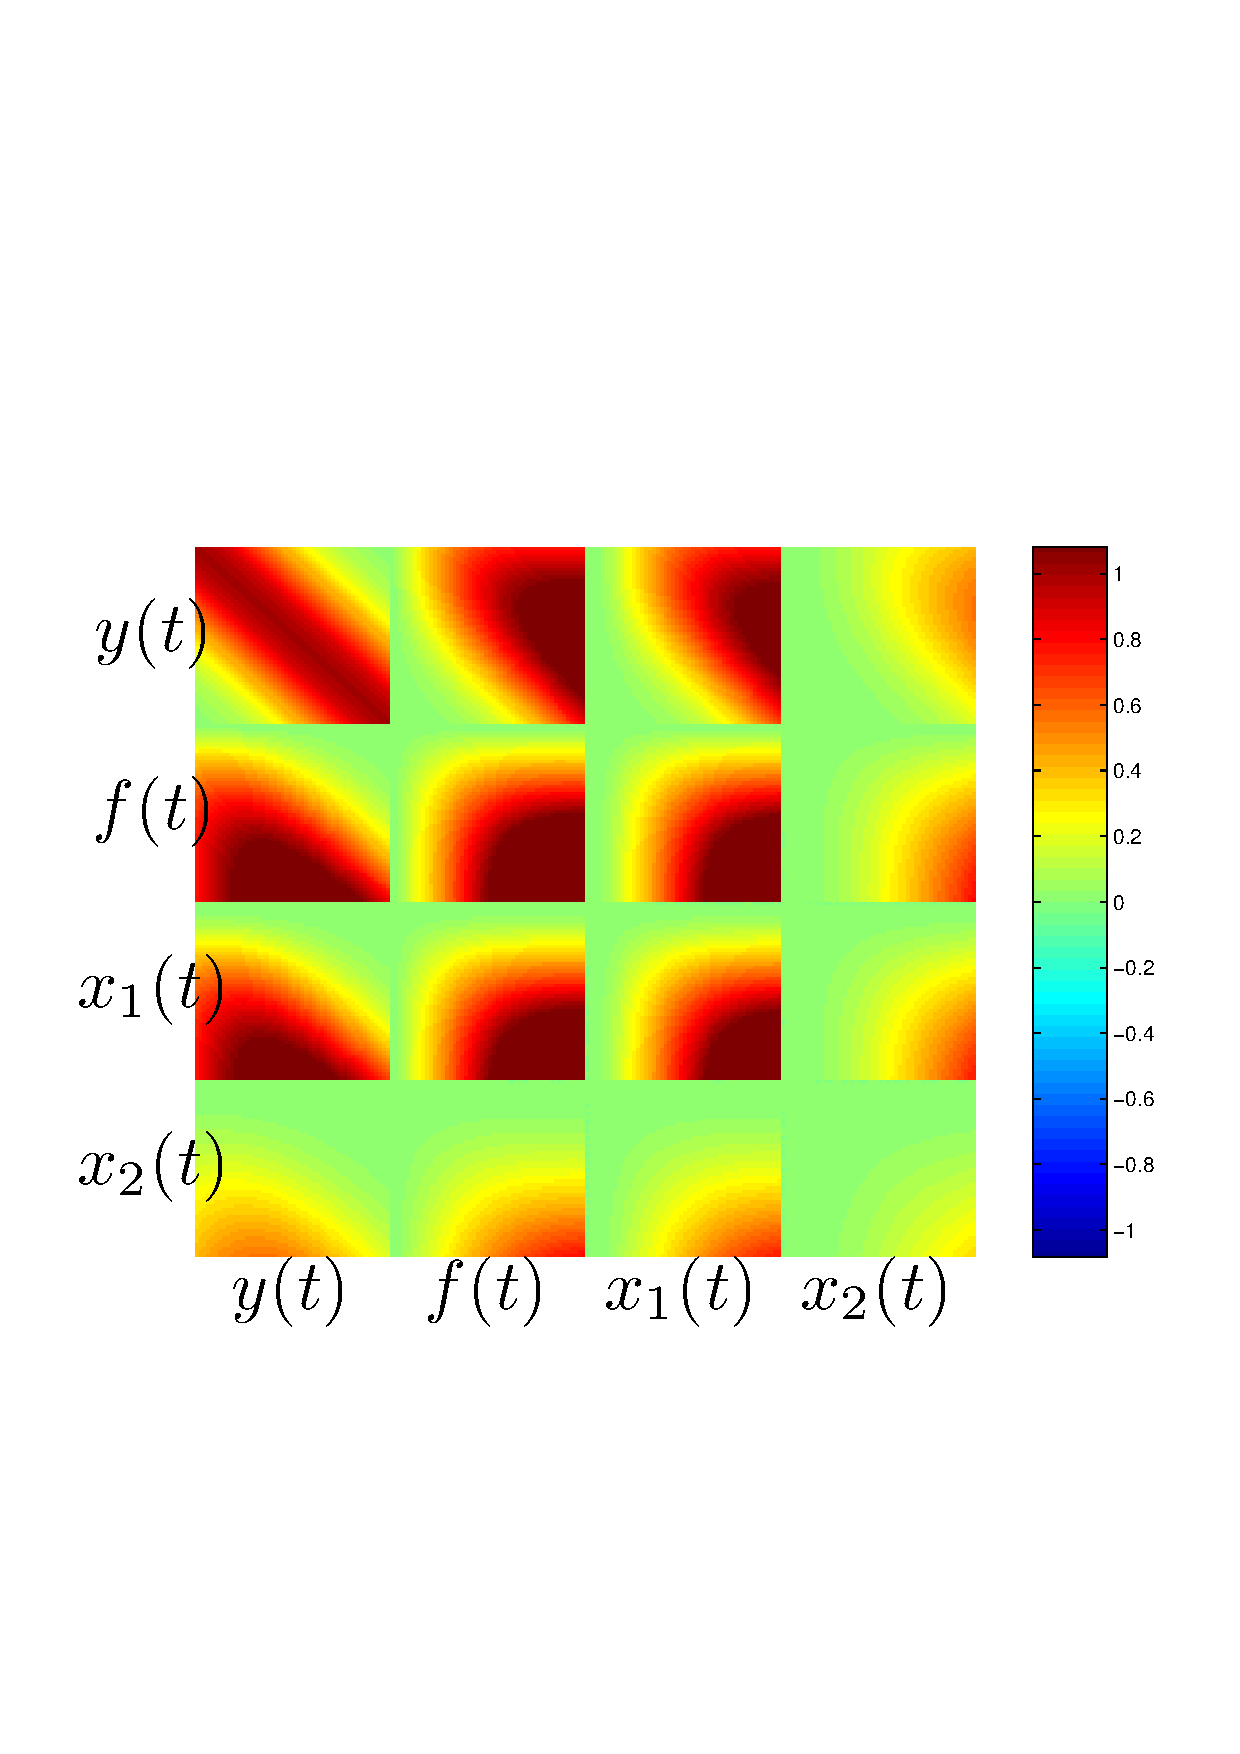
\includegraphics[width=0.8\columnwidth]{../../../gpsim/tex/diagrams/gpdisimTestKernelImage}
      \par\end{center}

  \end{columns}

\end{frame}

\begin{frame}
  \frametitle{Results for Mef2 using the Cascade model}
  \begin{columns}[c]


    \column{2 in}

    % 
    \begin{figure}
      \centering{} 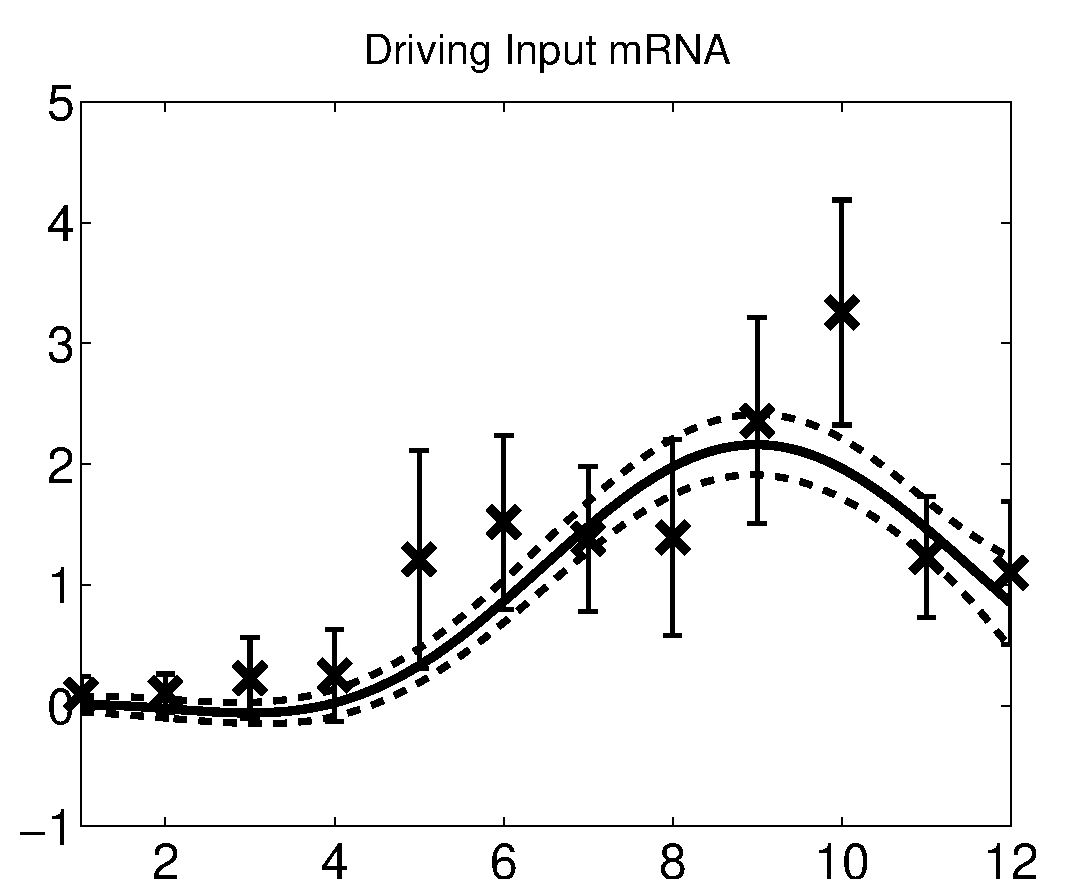
\includegraphics[width=4cm]{../../../gpsim/tex/diagrams/demMef2_ExprsProfile_Rep1_Gene1} 
    \end{figure}


    % 
    \begin{figure}
      \centering{} 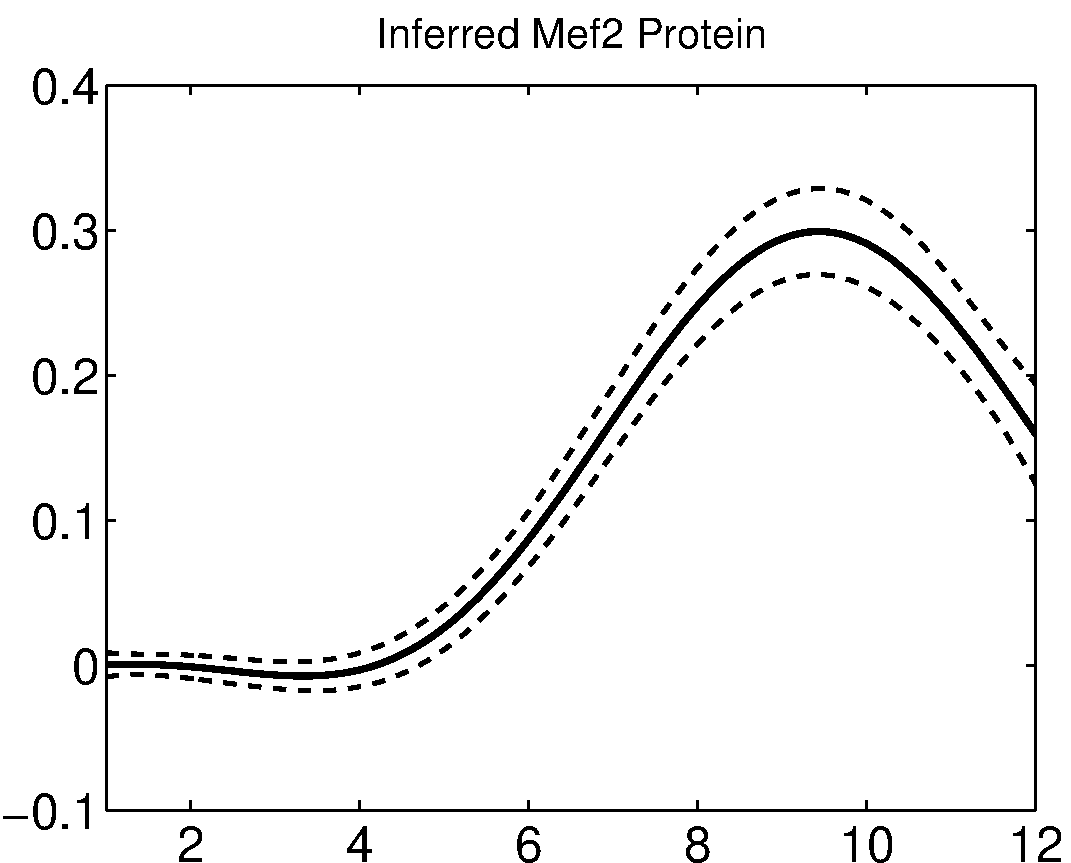
\includegraphics[width=4cm]{../../../gpsim/tex/diagrams/demMef2TF_profile_Rep1}
    \end{figure}


    \centering


    \column{2 in}

    % 
    \begin{figure}
      \centering{} 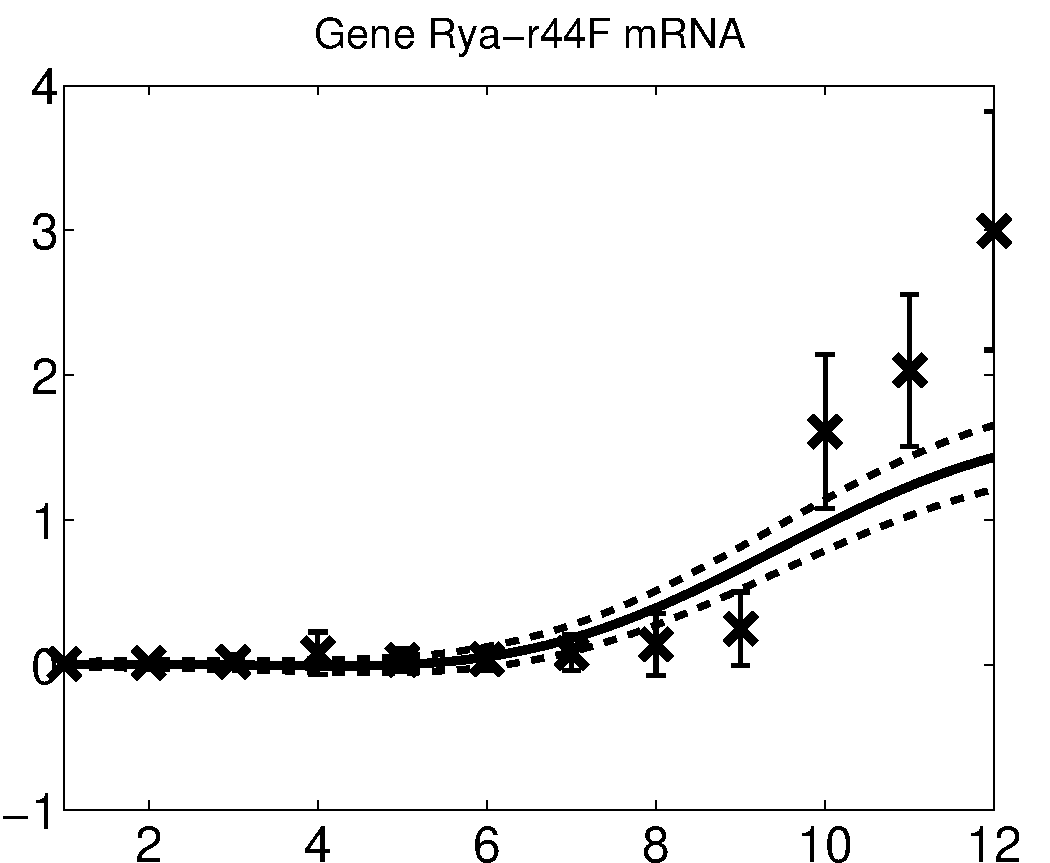
\includegraphics[width=4cm]{../../../gpsim/tex/diagrams/demMef2_ExprsProfile_Rep1_Gene2} 
    \end{figure}


    % 
    \begin{figure}
      \centering{} 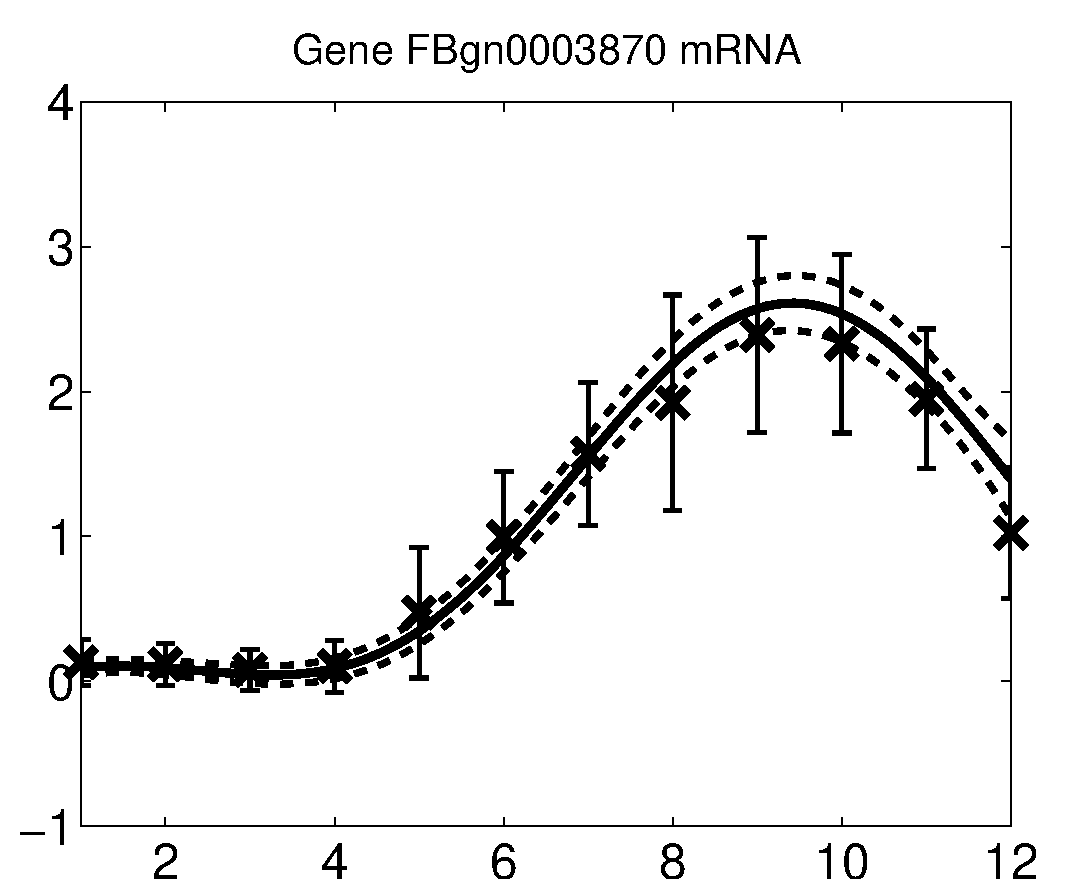
\includegraphics[width=4cm]{../../../gpsim/tex/diagrams/demMef2_ExprsProfile_Rep1_Gene4} 
    \end{figure}


  \end{columns}

\end{frame}

